\documentclass[11pt]{article}
\usepackage[ngerman]{babel}
\usepackage[utf8]{inputenc}
\usepackage{graphicx}
\graphicspath{ {graphics/} }

\begin{document}

\begin{titlepage}
\newcommand{\HRule}{\rule{\linewidth}{0.5mm}} % Defines a new command for the horizontal lines, change thickness here

\center 

\textsc{\LARGE Karlsruher Institut für Technologie}\\[1.5cm] % Name of your university/college
\textsc{\Large Proseminar}\\[0.5cm] % Major heading such as course name
\textsc{\large Informatik in der Medizin}\\[0.5cm] % Minor heading such as course title

\HRule \\[0.4cm]
{ \huge \bfseries Mechanische Eigenschaften von Weichgewebe}\\[0.4cm] % Title of your document
{ \LARGE Gliederung}\\[0.4cm]
\HRule \\[1.5cm]
 

\begin{minipage}{0.4\textwidth}
\begin{flushleft} \large
\emph{Autor:}\\
 Lena Winter 
\end{flushleft}
\end{minipage}
~
\begin{minipage}{0.4\textwidth}
\begin{flushright} \large
\emph{Betreuer:} \\
Jan Hergenhan
\end{flushright}
\end{minipage}\\[4cm]


%----------------------------------------------------------------------------------------
%	DATE SECTION
%----------------------------------------------------------------------------------------

{\large \today}\\[3cm] % Date, change the \today to a set date if you want to be precise

%----------------------------------------------------------------------------------------
%	LOGO SECTION
%----------------------------------------------------------------------------------------

%\includegraphics{Logo}\\[1cm] % Include a department/university logo - this will require the graphicx package
 
%----------------------------------------------------------------------------------------

\vfill % Fill the rest of the page with whitespace

\end{titlepage}
	\section{Motivation:}
		Durch die Entwicklungen in den Gebieten der Robotik, Mechanik und Medizin konnte in den 
		letzten Jahren erreicht werden, dass weltweit in den Operationssäle vermehrt
		rechnergestützte Operationssysteme zum Einsatz kommen. Diese dienen dazu menschliche 
		Chirugen zu unterstützen und ihnen zu größere Genauigkeit bei Operationen zu verhelfen. 
		Allerdings fehlen diesen Systemen wichtige Modelle die menschliche Chirugen verinnerlicht
		haben, so zum Beispiel wie sich Weichgewebe wie Organe bei Krafteinwirkung durch 
		Instrumente verhält. Um den Chirugen, die das System steuern ein umfassendes Bild der 
		vorliegenden Situation und bessere Planbarkeit bei Operationsschritten zu bieten, ist es 
		deshalb wichtig auch die mechanischen Eigenschaften der verschiedenen Gewebearten in 
		geeigneten Modellen zu beschreiben und die zugehörigen Parameter zu bestimmen. Dadurch wird 
		es möglich diese Modelle in die Operationssysteme einzugliedern um dadurch ihre Handhabung 
		zu vereinfachen.
	
		   
	\section{Grundlagen:}
	
		Weichgewebe haben im Allgemeinen viskoeslastische Eigeschaften. Diese setzten sich aus drei 
		wesentlichen Effekten zusammen, der Hysterese, der Relaxion und des Kriechens. Das
		Verhalten, das man bei Be- und Entlastung, verschiedenes  Spannung-Dehnungsverhalten
		beobachten kann nennt man Hysterese. Als Relaxation bezeichnet man das Verhalten, dass 
		sich unter konstanter Spannung in einem Körper, eine konstante Dehnung einstellt. Wenn sich 
		bei einem Körper unter konstanter Spannung eine fortschreitende Deformation zeigt nennt man
		dieses Verhalten Kriechen.
		
		\begin{figure}[h!]
		  \centering
			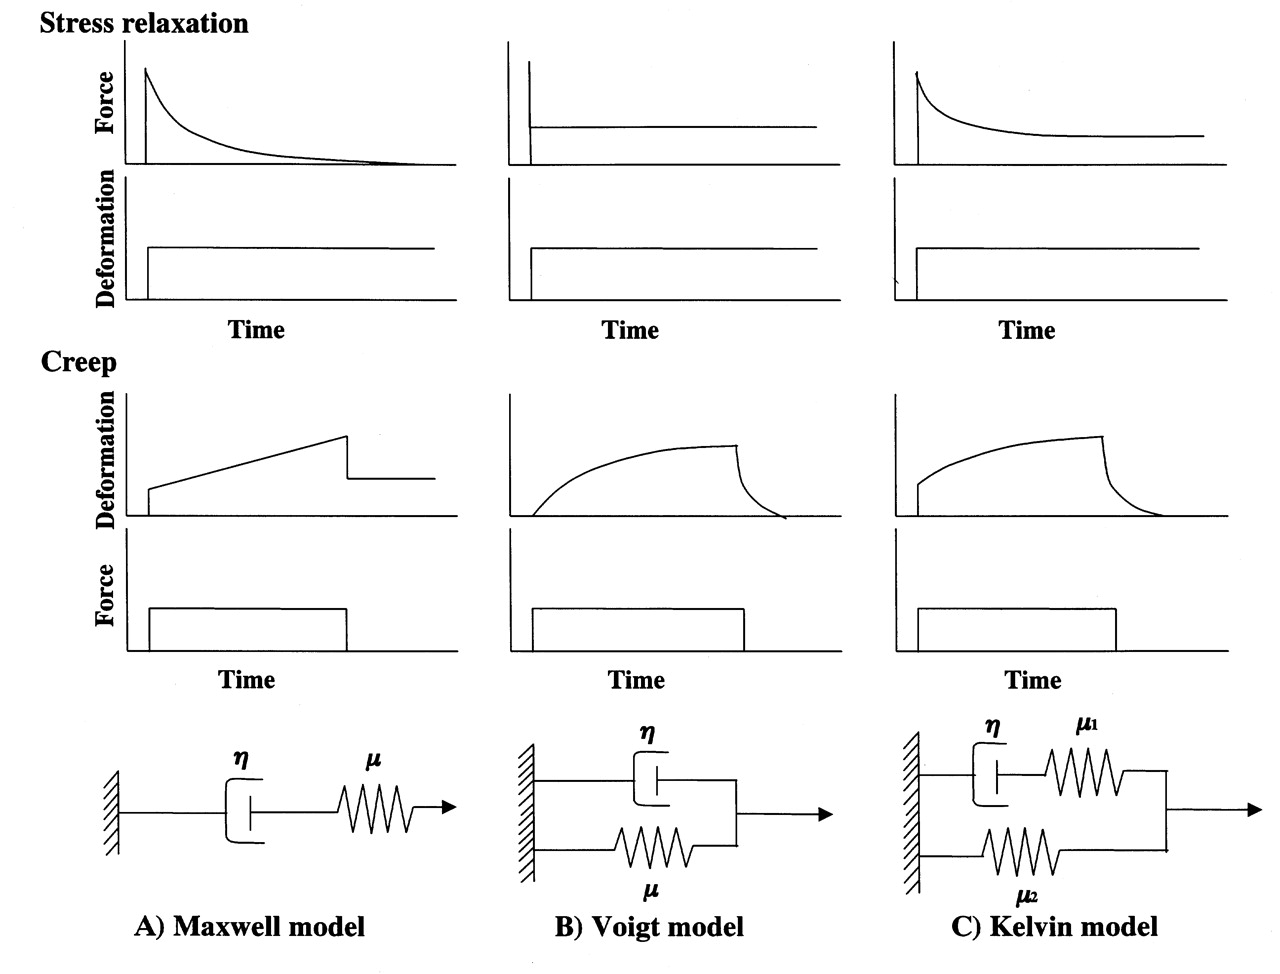
\includegraphics[width=\textwidth]{viskomod.jpg}
			\caption{Mechanische Modelle für viskoelastisches Verhalten für  Relaxation und Kriechen.}
		\end{figure}
		
		Um diese drei Effekte der Viskoelastizität darzustellen gibt es verschiedene mechanische 
		Modelle. Die drei gängisten dieser Modelle sind der MAXWELL-, der VOIGT- und der KELVIN-
		Körper. Diese Modelle bestehen aus verschiedenen Zusammenstellungen von Federn und Dämpfern.
		In Abbildung 1 werden alle drei Modelle mit Zeit-Kraft- bzw. Zeit-Deformations-Diagrammen 
		dargestellt. 
		
		

		 

	\section{Messverfahren: Oszillationsversuch}
		 Zu den Parametern die bestimmt werden müssen gehört auch die Impedanz des Gewebes.
		 Dabei handelt es sich um den Wiederstand den das Gewebe Welle bietet die sich darin 
		 ausbreiten. Um einen solchen Parametern korrekt zu bestimmen sind mehrere Versuche nötig 
		 die mit Wellen verschiedener Amplituden und Frequenzen arbeiten. Exemplarisch soll
		 hier der Versuchsaufbau eines Messplatzes im Frequenzbereich bis 50 Hz mit maximaler 
		 Wegamplitude von 15 mm erläutert werden. Dieser Messplatz dient dazu, die Impedanz des 
		 Gewebes bei niederfrequenter kinästhetischer Manipulation zu messen.
		  
		 \begin{figure}[h!]
		  \centering
			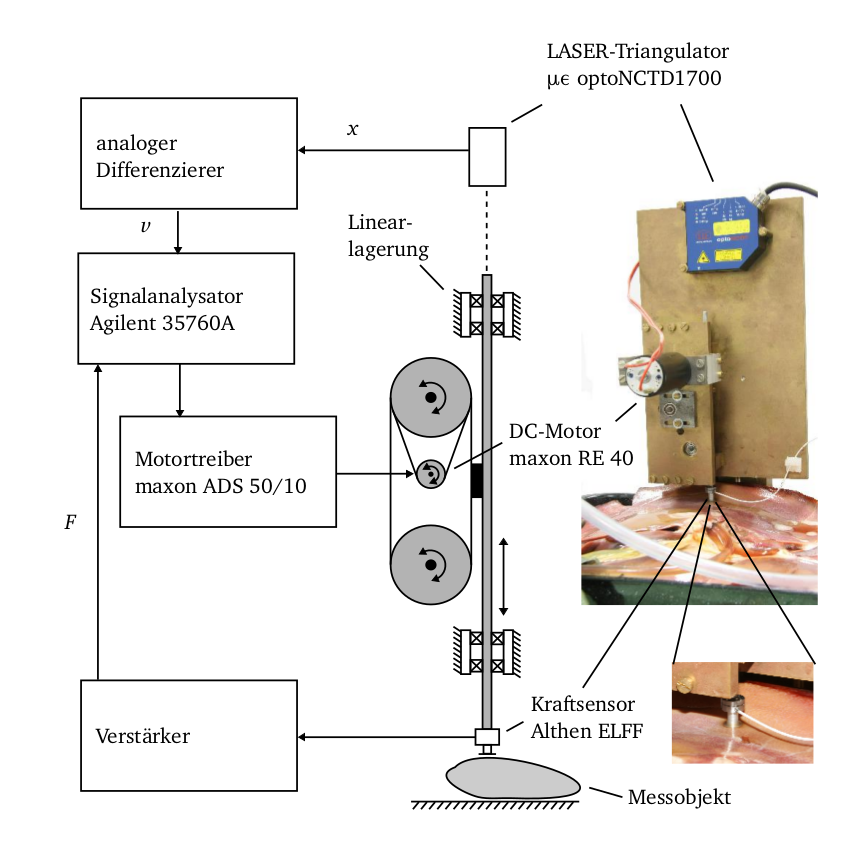
\includegraphics[width=\textwidth]{mess2.png}
			\caption{Schematischer Aufbau des Messplatzes.}
		\end{figure} 
		
		 Die mechanische Stimulation des Gewebes erfolgt dabei über ein Seil-Rollengetriebe, das 
		 die rotorische Oszillation eines Elektomotors in eine translatorische Oszillations 	
		 überführt, die dann durch einen Strößel mit Durchmesser 8mm auf das Gewebe übertragen 
		 wird. Es wird wärend des Versuches durch Lasertriangulation die Geschwindigkeitsantwort 
		 des Messobjektes gemessen. Die auf das 
		 Messobjekt angewandte Kraft wird durch einen Kraftsensor aufgezeichnet. Als Messobjekt 
		 dient in diesem Versuch eine Schweineleber, die sich sehr ähnlich zu menschlichem Gewebe 
		 verhält. Um über mehrere Stunden die gleichen Vorrausetzungen bieten zu können und um die 
		 Ergebnisse der Messung so nah wie möglich an den Werten von lebenden Organen zu halten, 
		 wird das Versuchsobjekt wärend des Versuches mit einer NaCl-Lösung künstlich durchblutet.
		 
		 Die Messung an einer Leber dauert in etwa sechs Stunden. Von den dabei erhaltenen 
		 Messwerten wird anschließend der Messplatzfehler abgezogen der im Leerlauf des Messplatzes 
		 ermittelt wird. Bei der Messung ergeben sich dann die in Abb 3 sichtbaren Ergebnisse. Bei 
		 dieser Messung wurde im Frequenzbereich von 0 bis 50 Hz  aufgezeichnet. Dabei ist bei 
		 in Abbildung 3 gut erkennbar das sich das Verhalten für kleine Frequenzen bis ca. 10 bis 	
		 20 Hz von dem für höhere Frequenzen unterscheidet. 
		 
		 Aus diesen experimentell gewonnenen Daten lassen sich nun Modelle für das Verhalten 
		 bestimmen. Als besonders geeignet haben sich hierfür elektrische Schaltungen mit 
		 verschiedenen Schaltungen von Kondensatoren und Widerständen erwiesen deren Schaltung 
		 und Werte durch Erfahrung und den Messwerten des Experimentes bestimmt werden können.
		  
		 
		 \begin{figure}[h!]
		  \centering
			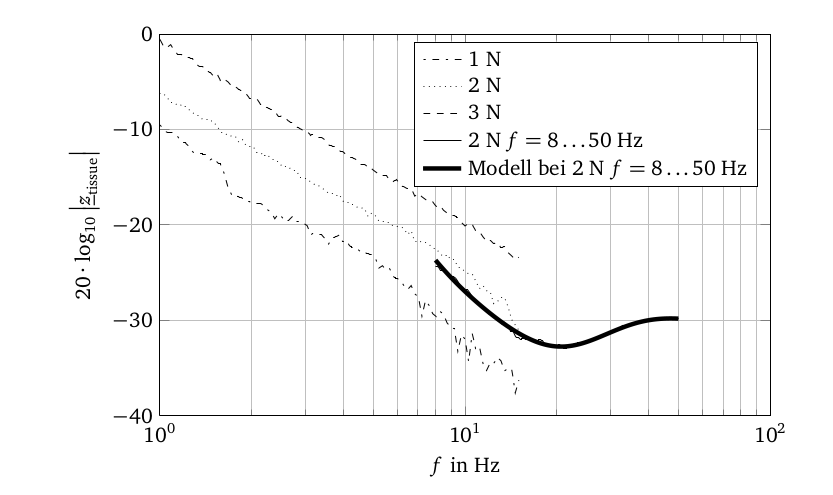
\includegraphics[width=\textwidth]{messerg.png}
			\caption{Messergebnisse: in y-Richtung ist die Impedanz in x-Richtung Fequenz aufgetragen.}
		\end{figure} 
		
	\section{Anwendung}
		 
		\subsection{Trainingsprogramme für minimal invasive Chrirugie:}
			Die minimal invasive Chirugie kommt seit dem Anfang der 90er Jahre zum Einsatz. Dabei
			wird, statt das Operationsgebiet, zumeist der Bauchraum, großflächig zu öffnen, mit 
			mehreren kleinen Einschnitten für die Instrumente. Der Nachteil an dieser Methode ist 
			allerdings das die in diesem Gebiet unerfahrenen Ärzte dies nicht einfach wie sonst
			üblich dadurch erlernen können einem erfahrenen Chirugen bei Operationen zu beobachten.
			In der Vergangenheit wurden deshalb zum Training von angehenden Chrirugen 
			und zum Trainieren neuer Techniken oft Organe von Tieren oder deren gesamter Körper 
			eingesetzt um solche Verfahren zu üben. Allerdings ist die Anatomie von einigen 
			Tieren, wie Schweinen, zwar änlich zu der menschlichen aber sicherlich nicht genau 
			gleich. Hinzukommen die Kosten für die Trainingsobjekte und deren anschließende 
			Entsorgung. Zusammengefasst lässt sich also sagen das diese Trainingsmethode sehr 
			teuer ist und dabei keine herausragende Effiziens bietet. 
			Aus diesen Gründen waren die Bemühungen sehr groß Trainingssysteme zu entwickeln die 
			kein echtes Gewebe mehr benötigen sondern dieses einfach simulieren. Solche Systeme 
			sind damit auf Dauer gesehen sowohl billiger als auch Umweltfreundlicher und können
			dem Trainierenden eine Realitäts getreue Simulation eines Menschlichen Körpers bieten.
			Desweiteren lassen sich bei einem Trainingssimulator auch Ausnahmesitutationen oder
			anatomische Besonderheiten darstellen.
			
			\begin{figure}[h!]
			  \centering
				\includegraphics[width=\textwidth]{vsone.jpg}
				\caption{VsOne System}
			\end{figure} 
			Eines dieser Trainingssysteme ist das 2001 entwickelte VSOne, welches sowohl haptisches 
			Feedback liefert als 
			auch virtuelle Modelle der Organe durch die Software KisMo liefert. Es liegt dem 
			System dabei eine Datenbank mit den experimentell bestimmten Parametern zu Grunde, die 
			bei der Modellierung der Organe verwendet werden. Wird durch den Trainierenden eine 
			Aktion an dem Organ ausgeführt, so werden die Parameter sowohl zur Berechnung des 
			Verhaltens des Organes, wie Deformation benutzt, als auch um den Widerstand 
			auszurechnen den ein solches Organ zum Beispiel bei einem Greifvorgang bietet.
			Dabei wird auf einem Bildschirm ein Bild der momentanen Situation in echtzeit 
			ausgegeben, wie es auch bei einer echten Operation geschehen würde.
			
		Dies ist nur eine Anwendung für die Bestimmten Parameter. Sie werden auch in weiteren 
		Programmen eingesetzt, so zum Beispiel um auch bei der robotergestützen Chirugie dem 
		Operierendem ein haptisches Feedback zu bieten. Auch Trainingsprogramme für 
		robotergestützte Chirugie werden mit diesen Parametern entwickelt.
			
 
			  

			
	\section{Fazit:}
		Durch die Bestimmung von Modellen und deren zugehöriger Parameter um die mechanischen
		Eigenschaften von Weichgewebe zu bestimmen und ihnen maschinenlesbare Form zu geben, hat
		man Erreicht das alte Technologien wie die Laproskopie heute sicherer und effizienter 
		trainiert werden können und einen wichtigen Baustein für die Weiterentwicklung und 
		Verbesserung von neuern Technologien wie der robotergestützen Chirugie geliefert.
		Durch diese und ähnliche Untersuchungen werden auch Zukunftstechnologien wie autonom
		operierende Roboter etwas wahrscheinlicher, da nun das Verhalten eines Organs bereits im 
		Vorfeld berechnet werden kann. 
		
		 
			  
			
	\section{Glossar:}
	\begin{itemize}
		\item Impedanz: Die Impedanz fasst alle Widerstände zusammen die Schwingungen entgegenwirken.
	\end{itemize}
			 
		  
\end{document}
